
%%%%%%%%%%%%%%%%%%%%%%%%%%%%%%%%%%%%%%%%%%%%%%%%%%%%%%%%%%%%%%%%%%%%%%%%%%%%%%
%                                                                            %
%  ************************** AVISO IMPORTANTE **************************    %
%                                                                            %
% Éste es un documento de ayuda para los autores que deseen enviar           %
% trabajos para su consideración en el Boletin de la Asociación Argentina    %
% de Astronomía.                                                             %
%                                                                            %
% Los comentarios en este archivo contienen instrucciones sobre el formato   %
% obligatorio del mismo que complementan los instructivos web y PDF.         %
% Por favor léalos.                                                          %
%                                                                            %
% No deben borrarse los comentarios en este archivo. En caso contrario,      %
% el sistema de recepción de manuscritos no permitirá el envío de su         %
% contribución. No se permite el uso de \newcommand ni definiciones          %
% particulares de cada autor.                                                %
%                                                                            %
%%%%%%%%%%%%%%%%%%%%%%%%%%%%%%%%%%%%%%%%%%%%%%%%%%%%%%%%%%%%%%%%%%%%%%%%%%%%%%

%%%%%%%%%%%%%%%%%%%%%%%%%%%%%%%%%%%%%%%%%%%%%%%%%%%%%%%%%%%%%%%%%%%%%%%%%%%%%%
%                                                                            %
%  ************************** IMPORTANT NOTICE **************************    %
%                                                                            %
%  This is a help file for authors who are preparing manuscripts to be       %
%  considered for publication in the Boletin de la Asociación Argentina      %
%  de Astronomía.                                                            %
%                                                                            %
%  The comments in this file give instructions about the manuscripts'        %
%  mandatory format that complement the instructions distributed as a PDF    %
%  and findable in the BAAA web. Please read them.                           %
%                                                                            %
%  The comments in this file must not be deleted. Otherwise, your            %
%  contribution will be rejected by the manuscript reception system.         %
%  The use of \newcommand and author definitions are forbidden.              %
%                                                                            %
%%%%%%%%%%%%%%%%%%%%%%%%%%%%%%%%%%%%%%%%%%%%%%%%%%%%%%%%%%%%%%%%%%%%%%%%%%%%%%

\documentclass[baaa]{baaa}

\usepackage[pdftex]{hyperref}
\usepackage{subfigure}
\usepackage{natbib}
\usepackage{helvet,soul}
\usepackage[font=small]{caption}
\usepackage{float}
\usepackage{graphicx}

%-------------------DEFINICIONES A REMOVER---------------------------
\def\Eeuv{E_{\rm{EUV}}}
\def\Ewl{E_{\rm{WL}}}
\def\AvgNE2{\left<N_e^2\right>}
\def\AvgNe{\left<N_e\right>}
\def\SigmaNe{\sigma_{Ne}}
\def\VarNe{\rm{Var}N_e}
\def\AvgTe{\left<T_e\right>}
\def\SigmaTe{\sigma_{Te}}
%---------------------------------------------------------------------

\begin{document}

%%%%%%%%%%%%%%%%%%%%%%%%%%%%%%%%%%%%%%%%%%%%%%%%%%%%%%%%%%%%%%%%%%%%%%%%%%%%%%
%                                                                            %
% Datos de la publicación, no deben ser cambiados.                           %
%                                                                            %
% Journal data, please do not change them.                                   %
%                                                                            %
%%%%%%%%%%%%%%%%%%%%%%%%%%%%%%%%%%%%%%%%%%%%%%%%%%%%%%%%%%%%%%%%%%%%%%%%%%%%%%

\journalvol{61A}
\journalyear{2019}
\journaleditors{R. Gamen, N. Padilla, C. Parisi, F. Iglesias \& M. Sgr\'o}

%%%%%%%%%%%%%%%%%%%%%%%%%%%%%%%%%%%%%%%%%%%%%%%%%%%%%%%%%%%%%%%%%%%%%%%%%%%%%%
%                                                                            %
%  Seleccione el idioma de su contribución: Recuerde que todos los           %
%  componentes del documento (titulo, texto, figuras, tablas, etc.)          %
%  deben estar en el mismo idioma.                                           %
%                                                                            %
%  Select the languague of your contribution: Please remember that all       %
%  document parts (title, text, figures, tables, etc.) must be in the        %
%  same languaje.                                                            %
%                                                                            %
%  0: Castellano / Spanish                                                   %
%  1: Inglés / English                                                       %
%                                                                            %
%%%%%%%%%%%%%%%%%%%%%%%%%%%%%%%%%%%%%%%%%%%%%%%%%%%%%%%%%%%%%%%%%%%%%%%%%%%%%%

\contriblanguage{1}

%%%%%%%%%%%%%%%%%%%%%%%%%%%%%%%%%%%%%%%%%%%%%%%%%%%%%%%%%%%%%%%%%%%%%%%%%%%%%%
%                                                                            %
%  Seleccione el tipo de contribución solicitada:                            %
%                                                                            %
%  Select the requested contribution type:                                   %
%                                                                            %
%  1: Presentación mural / Poster                                            %
%  2: Presentación oral / Oral contribution                                  %
%  3: Informe invitado / Invited report                                      %
%  4: Mesa redonda / Round table                                             %
%  5: Presentación Premio Varsavsky / Varsavsky Prize contribution           %
%  6: Presentación Premio Sahade / Sahade Prize contribution                 %
%  7: Presentación Premio Sérsic / Sérsic Prize contribution                 %
%                                                                            %
%%%%%%%%%%%%%%%%%%%%%%%%%%%%%%%%%%%%%%%%%%%%%%%%%%%%%%%%%%%%%%%%%%%%%%%%%%%%%%

\contribtype{2}

%%%%%%%%%%%%%%%%%%%%%%%%%%%%%%%%%%%%%%%%%%%%%%%%%%%%%%%%%%%%%%%%%%%%%%%%%%%%%%
%                                                                            %
%  Seleccione el área temática de su contribución:                           %
%                                                                            %
%  Select the thematic area of your contribution:                            %
%                                                                            %
%  1 [AEC]: Astrofísica Extragaláctica y Cosmología /                        %
%           Extragalactic Astrophysics and Cosmology                         %
%  2 [EG]: Estructura Galáctica / Galactic Structure                         %
%  3 [AE]: Astrofísica Estelar / Stellar Astrophysics                        %
%  4 [SE]: Sistemás Estelares / Stellar Systems                              %
%  5 [ICSA]: Instrumentación y Caracterización de Sitios Astronómicos /      %
%            Instrumentation and Astronomical Site Characterization          %
%  6 [MI]: Medio Interestelar / Interstellar Medium                          %
%  7 [OCPAE]: Objetos Compactos y Procesos de Altas Energías /               %
%             Compact Objetcs and High-Energy Processes                      %
%  8 [SH]: Sol y Heliosfera / Sun and Heliosphere                            %
%  9 [SSE]: Sistemas Solar y Extrasolares / Solar and Extrasolar Systems     %
%  10 [HEDA]: Historia, Enseñanza y Divulgación de la Astronomía /           %
%             History, Teaching and Spreading of Astronomy                   %
%  11 [O]: Otros / Other Topics                                              %
%                                                                            %
%%%%%%%%%%%%%%%%%%%%%%%%%%%%%%%%%%%%%%%%%%%%%%%%%%%%%%%%%%%%%%%%%%%%%%%%%%%%%%

\thematicarea{8}

\title{Tomography of the Solar Corona with Multiple Instruments:\\ First Steps}
\subtitle{}

%%%%%%%%%%%%%%%%%%%%%%%%%%%%%%%%%%%%%%%%%%%%%%%%%%%%%%%%%%%%%%%%%%%%%%%%%%%%%%
%                                                                            %
%  Agregue un título corto para el encabezado de las páginas pares.          %
%                                                                            %
%  Add a short title to appear in the header of even pages.                  %
%                                                                            %
%%%%%%%%%%%%%%%%%%%%%%%%%%%%%%%%%%%%%%%%%%%%%%%%%%%%%%%%%%%%%%%%%%%%%%%%%%%%%%

\titlerunning{Multi-instrument Tomography}

%%%%%%%%%%%%%%%%%%%%%%%%%%%%%%%%%%%%%%%%%%%%%%%%%%%%%%%%%%%%%%%%%%%%%%%%%%%%%%
%                                                                            %
%  Lista de autores. Los nombres de los autores deben estar separados por    %
%  comas, y deben tener el formato A.E. Autor (iniciales apellido(s);   sin  %
%  coma entre apellido e iniciales ni espacios entre las iniciales).         %
%                                                                            %
%  Author list. Authors' names must be separated by commas, and stick to     %
%  the format A.E. Author (initials Family name -neither commas between      %
%  name and the initials nor blanks between the initials).                   %
%                                                                            %
%%%%%%%%%%%%%%%%%%%%%%%%%%%%%%%%%%%%%%%%%%%%%%%%%%%%%%%%%%%%%%%%%%%%%%%%%%%%%%

\author{D.G. Lloveras\inst{1}, A.M. Vásquez\inst{1,2}, Enrico Landi\inst{3}, Richard A. Frazin\inst{3} }
\authorrunning{Lloveras et al.}  
%%%%%%%%%%%%%%%%%%%%%%%%%%%%%%%%%%%%%%%%%%%%%%%%%%%%%%%%%%%%%%%%%%%%%%%%%%%%%%
%                                                                            %
% Por favor provea una dirección de e-mail de contacto para los lectores.    %
%                                                                            %
% Please provide a contact e-mail address for the readers.                   %
%                                                                            %
%%%%%%%%%%%%%%%%%%%%%%%%%%%%%%%%%%%%%%%%%%%%%%%%%%%%%%%%%%%%%%%%%%%%%%%%%%%%%%

\contact{dlloveras@iafe.uba.ar}

\institute{
  Insituto de Astronomía y Física del Espacio, CONICET--UBA, Argentina \and
  Departamento de Ciencia y Tecnología, UNTREF, Argentina \and
  Department of Climate ande Space Sciences and Engineering, University of Michigan, USA
}

%%%%%%%%%%%%%%%%%%%%%%%%%%%%%%%%%%%%%%%%%%%%%%%%%%%%%%%%%%%%%%%%%%%%%%%%%%%%%%
%                                                                            %
%  El resumen y el abstract son ambos obligatorios, independientemente del   %
%  lenguaje elegido.                                                         %
%                                                                            %
%  The Resumen and the abstract are both mandatory, regardless of the chosen %
%  language.                                                                 %
%                                                                            %
%%%%%%%%%%%%%%%%%%%%%%%%%%%%%%%%%%%%%%%%%%%%%%%%%%%%%%%%%%%%%%%%%%%%%%%%%%%%%%

\resumen{La tomografía solar rotacional es una técnica observacional de la corona solar que permite la reconstruccion de la distribución tri-dimensional (3D) global de algunos de sus parámetros fundamentales, como por ejemplo la densidad electrónica.  La tomografía basada en EUV es aplicada regularmente a datos obtenidos con telescopios espaciales, cubriendo típicamente el rango de alturas heliocéntricas $1.02-1.25~\rm{R}_\odot$. Este rango solapa parcialmente el del campo de visión del coronógrafo de luz blanca K-coronagraph (KCOR), en el High Altitude Observatory (HAO), que cubre el rango $1.05-3.0~\rm{R}_\odot$. En este trabajo presentamos resultados preliminares de la primer comparación de una reconstrucción de la densidad electrónica coronal obtenida utilizando imágenes EUV con la obtenida utilizando imágenes en luz blanca. Los resultados obtenidos son discutidos en términos de las diversas características de los datos utilizados, asi como de los diferentes factores físicos que afectan cada análisis. }

\abstract{Solar rotational tomography is an observational technique of the solar corona that allows reconstruction of the global three-dimensional distribution of some of its fundamental physical parameters, such as electron density. EUV tomography is routinely applied to data provided by spaceborne telescopes, typically covering the range of heliocentric heights $\approx 1.02-1.25~\rm{R}_\odot$. This range partially overlaps that of the field of view of the white light K-coronagraph (KCOR) instrument, at the High Altitude Observatory (HAO), which covers the range $\approx 1.05-3.0~\rm{R}_\odot$. In this work we show preliminary results of the first comparison of tomographic reconstruction of the coronal electron density based on EUV images against that reconstructed based on white light images. Results are discussed in terms of the diverse characteristics of the used data sets, as well as the different physical factors that affect each analysis.}

%%%%%%%%%%%%%%%%%%%%%%%%%%%%%%%%%%%%%%%%%%%%%%%%%%%%%%%%%%%%%%%%%%%%%%%%%%%%%%
%                                                                            %
%  Seleccione las palabras clave que describen su contribución. Las mismas   %
%  son obligatorias, y deben tomarse de la lista de la American Astronomical %
%  Society (AAS), que se encuentra en la página web indicada abajo.          %
%                                                                            %
%  Select the keywords that describe your contribution. They are mandatory,  %
%  and must be taken from the list of the American Astronomical Society      %
%  (AAS), which is available at the webpage quoted below.                    %
%                                                                            %
%  https://aas.org/authors/astronomical-subject-keywords-update-august-2013  %
%                                                                            %
%%%%%%%%%%%%%%%%%%%%%%%%%%%%%%%%%%%%%%%%%%%%%%%%%%%%%%%%%%%%%%%%%%%%%%%%%%%%%%

\keywords{Sun: corona --- Sun: fundamental parameters --- Sun: UV radiation --- Sun: abundances}

\maketitle

\section{Introduction}\label{intro}

Solar rotational tomography (SRT) was initially developed by \citet{altschuler_1972} for reconstruction of the three-dimensional (3D) distribution of the coronal electron density based on white light (WL) data. \citet{frazin_2002} developed a modern, robust, regularized, positive method for tomographic inversion of the coronal electron density from WL data, used in this work. A thorough review on WL tomography can be found in those references.

More recently, \citet{frazin_2009} developed the differential emission measure tomography (DEMT) technique. DEMT combines EUV tomography in several pass-bands with local DEM analysis, to reconstruct the 3D distribution of both the coronal electron density and temperature. A recent review by \citet{vasquez_2016} summarizes the existing solar physics literature based on DEMT analysis. More recent DEMT-based works include \citet{lloveras_2017}, who carried out a comparative analysis of the coronal structure at the solar minima between solar cycles (SC-)22/23 and 23/24.

DEMT research has been carried out based on data provided by several generations of spaceborne EUV telescopes. The latest one is the Atmospheric Imaging Assembly (AIA) instrument, on board the Solar Dynamics Observatory (SDO), whose data is used in this work.

\begin{figure*}[h]
  \centering
  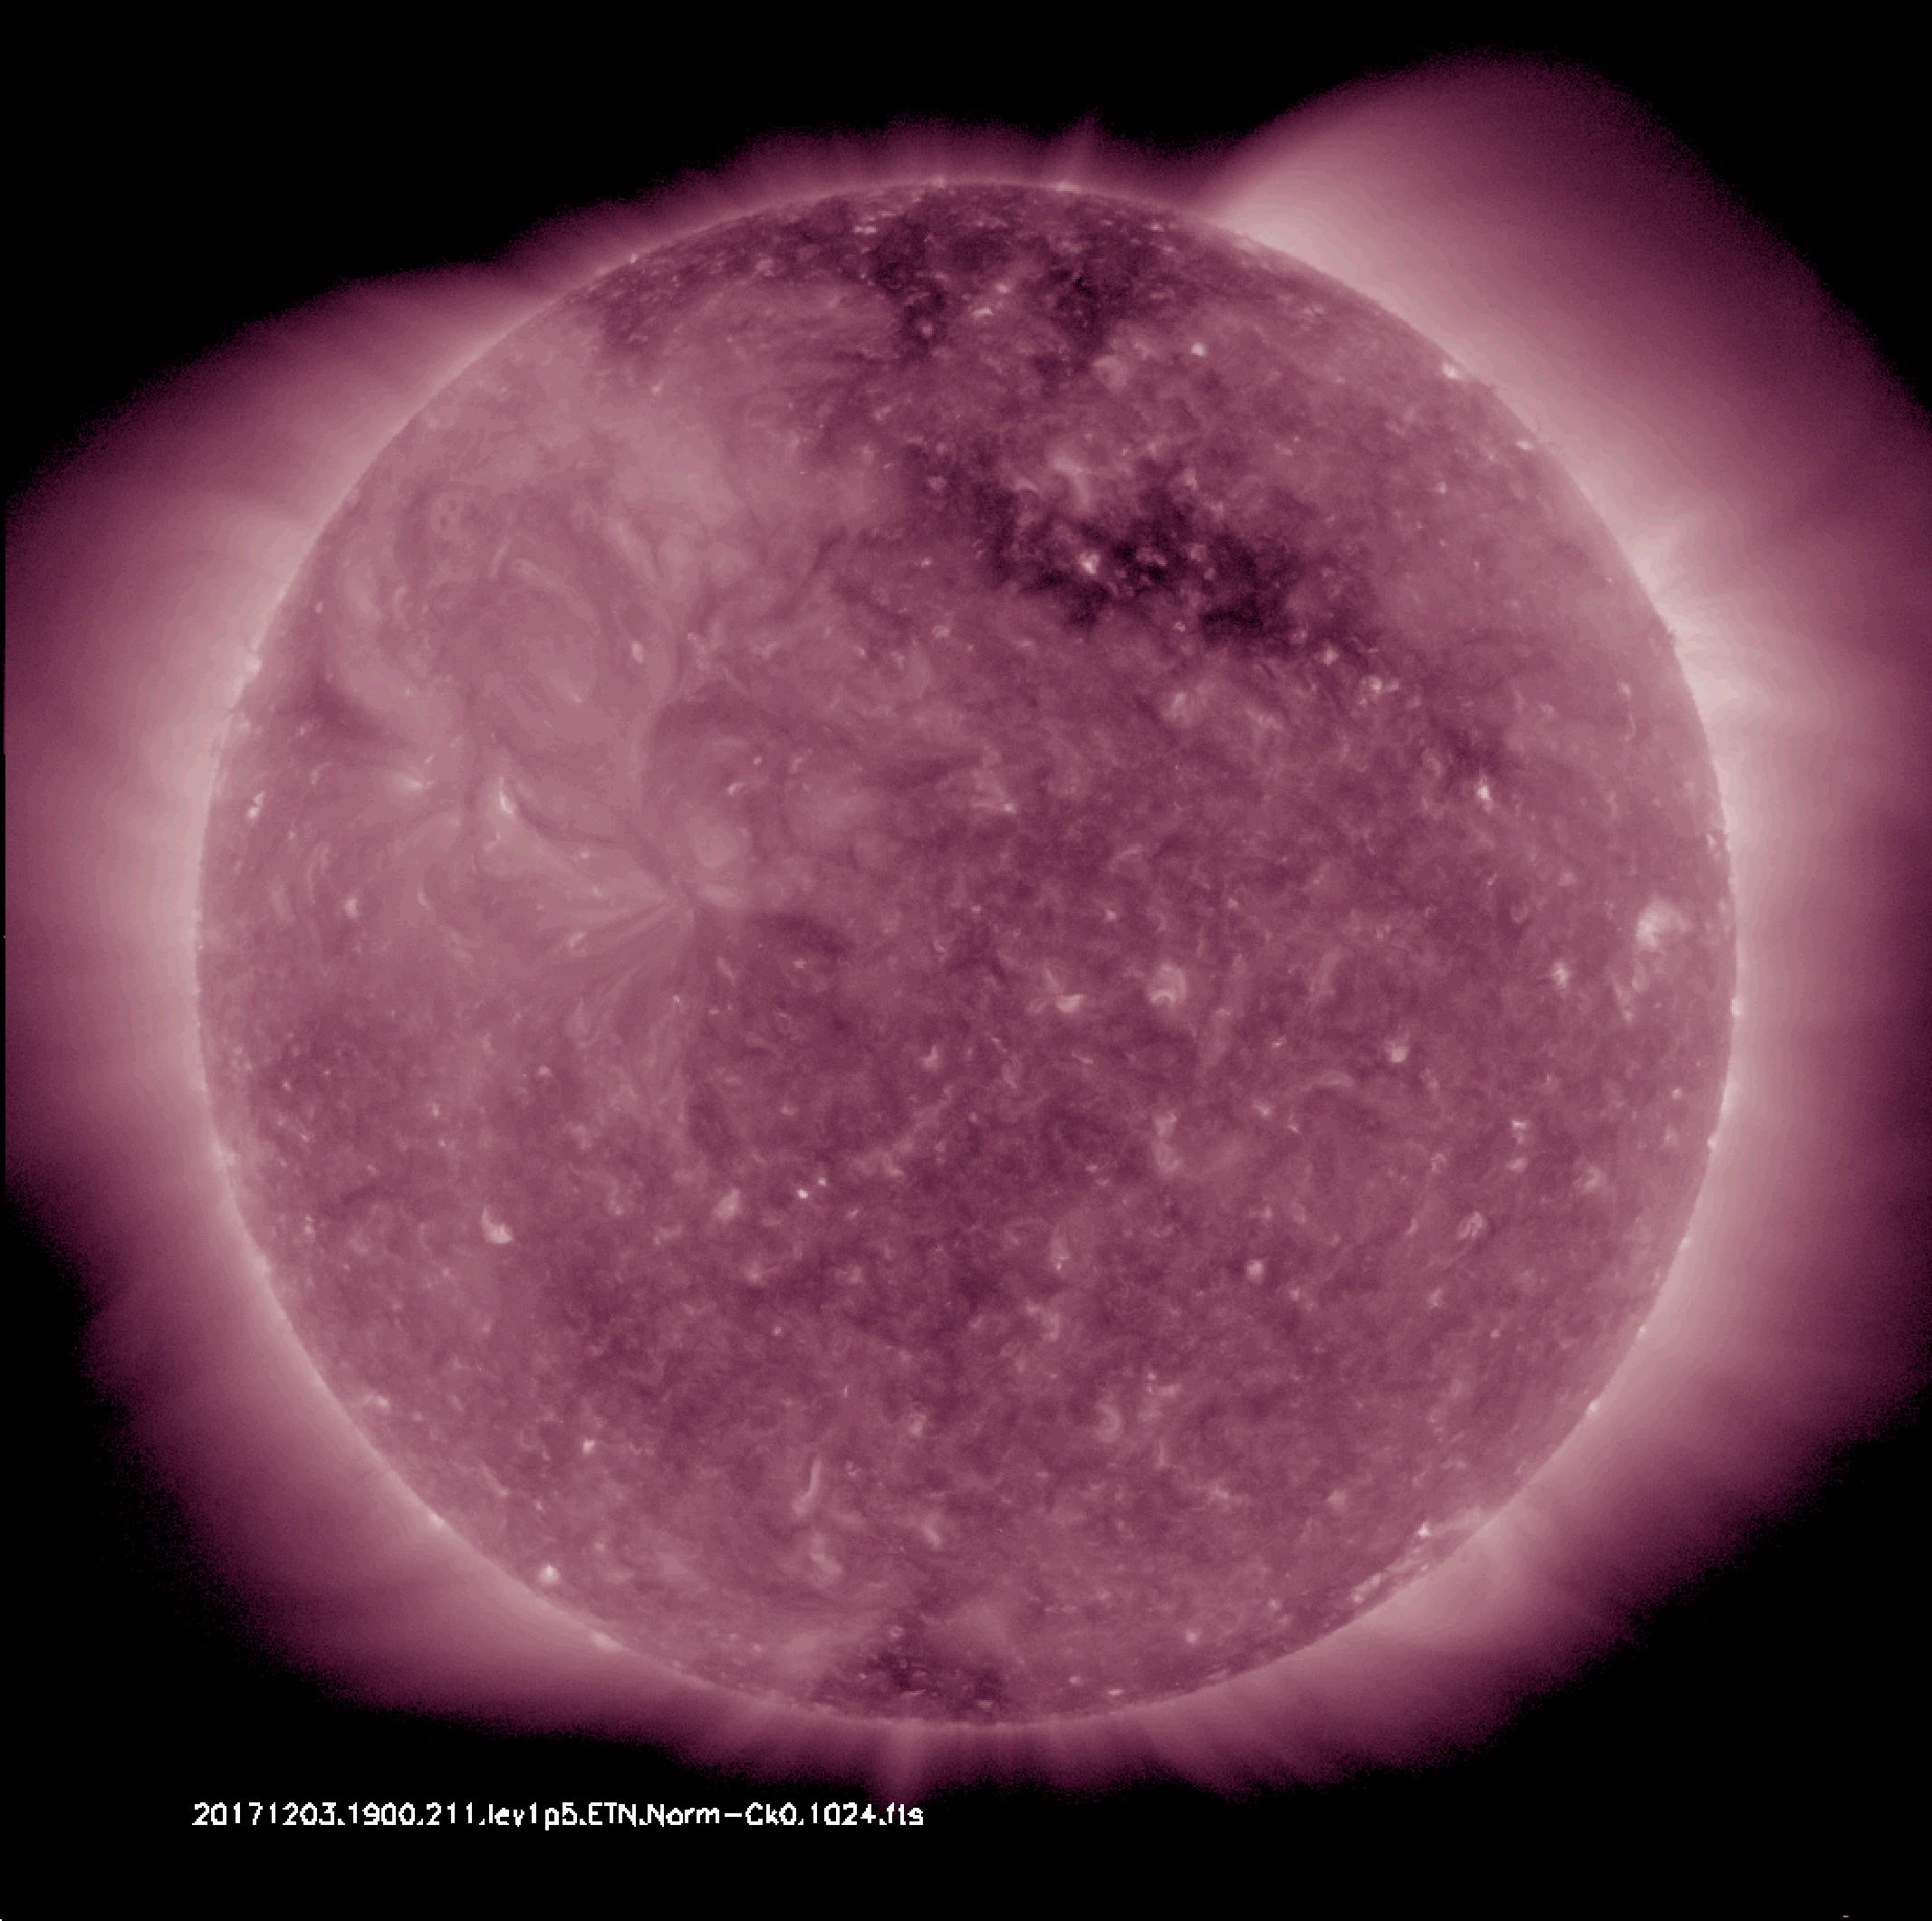
\includegraphics[width=0.68\columnwidth]{img_211.pdf}
  \hskip 1cm
  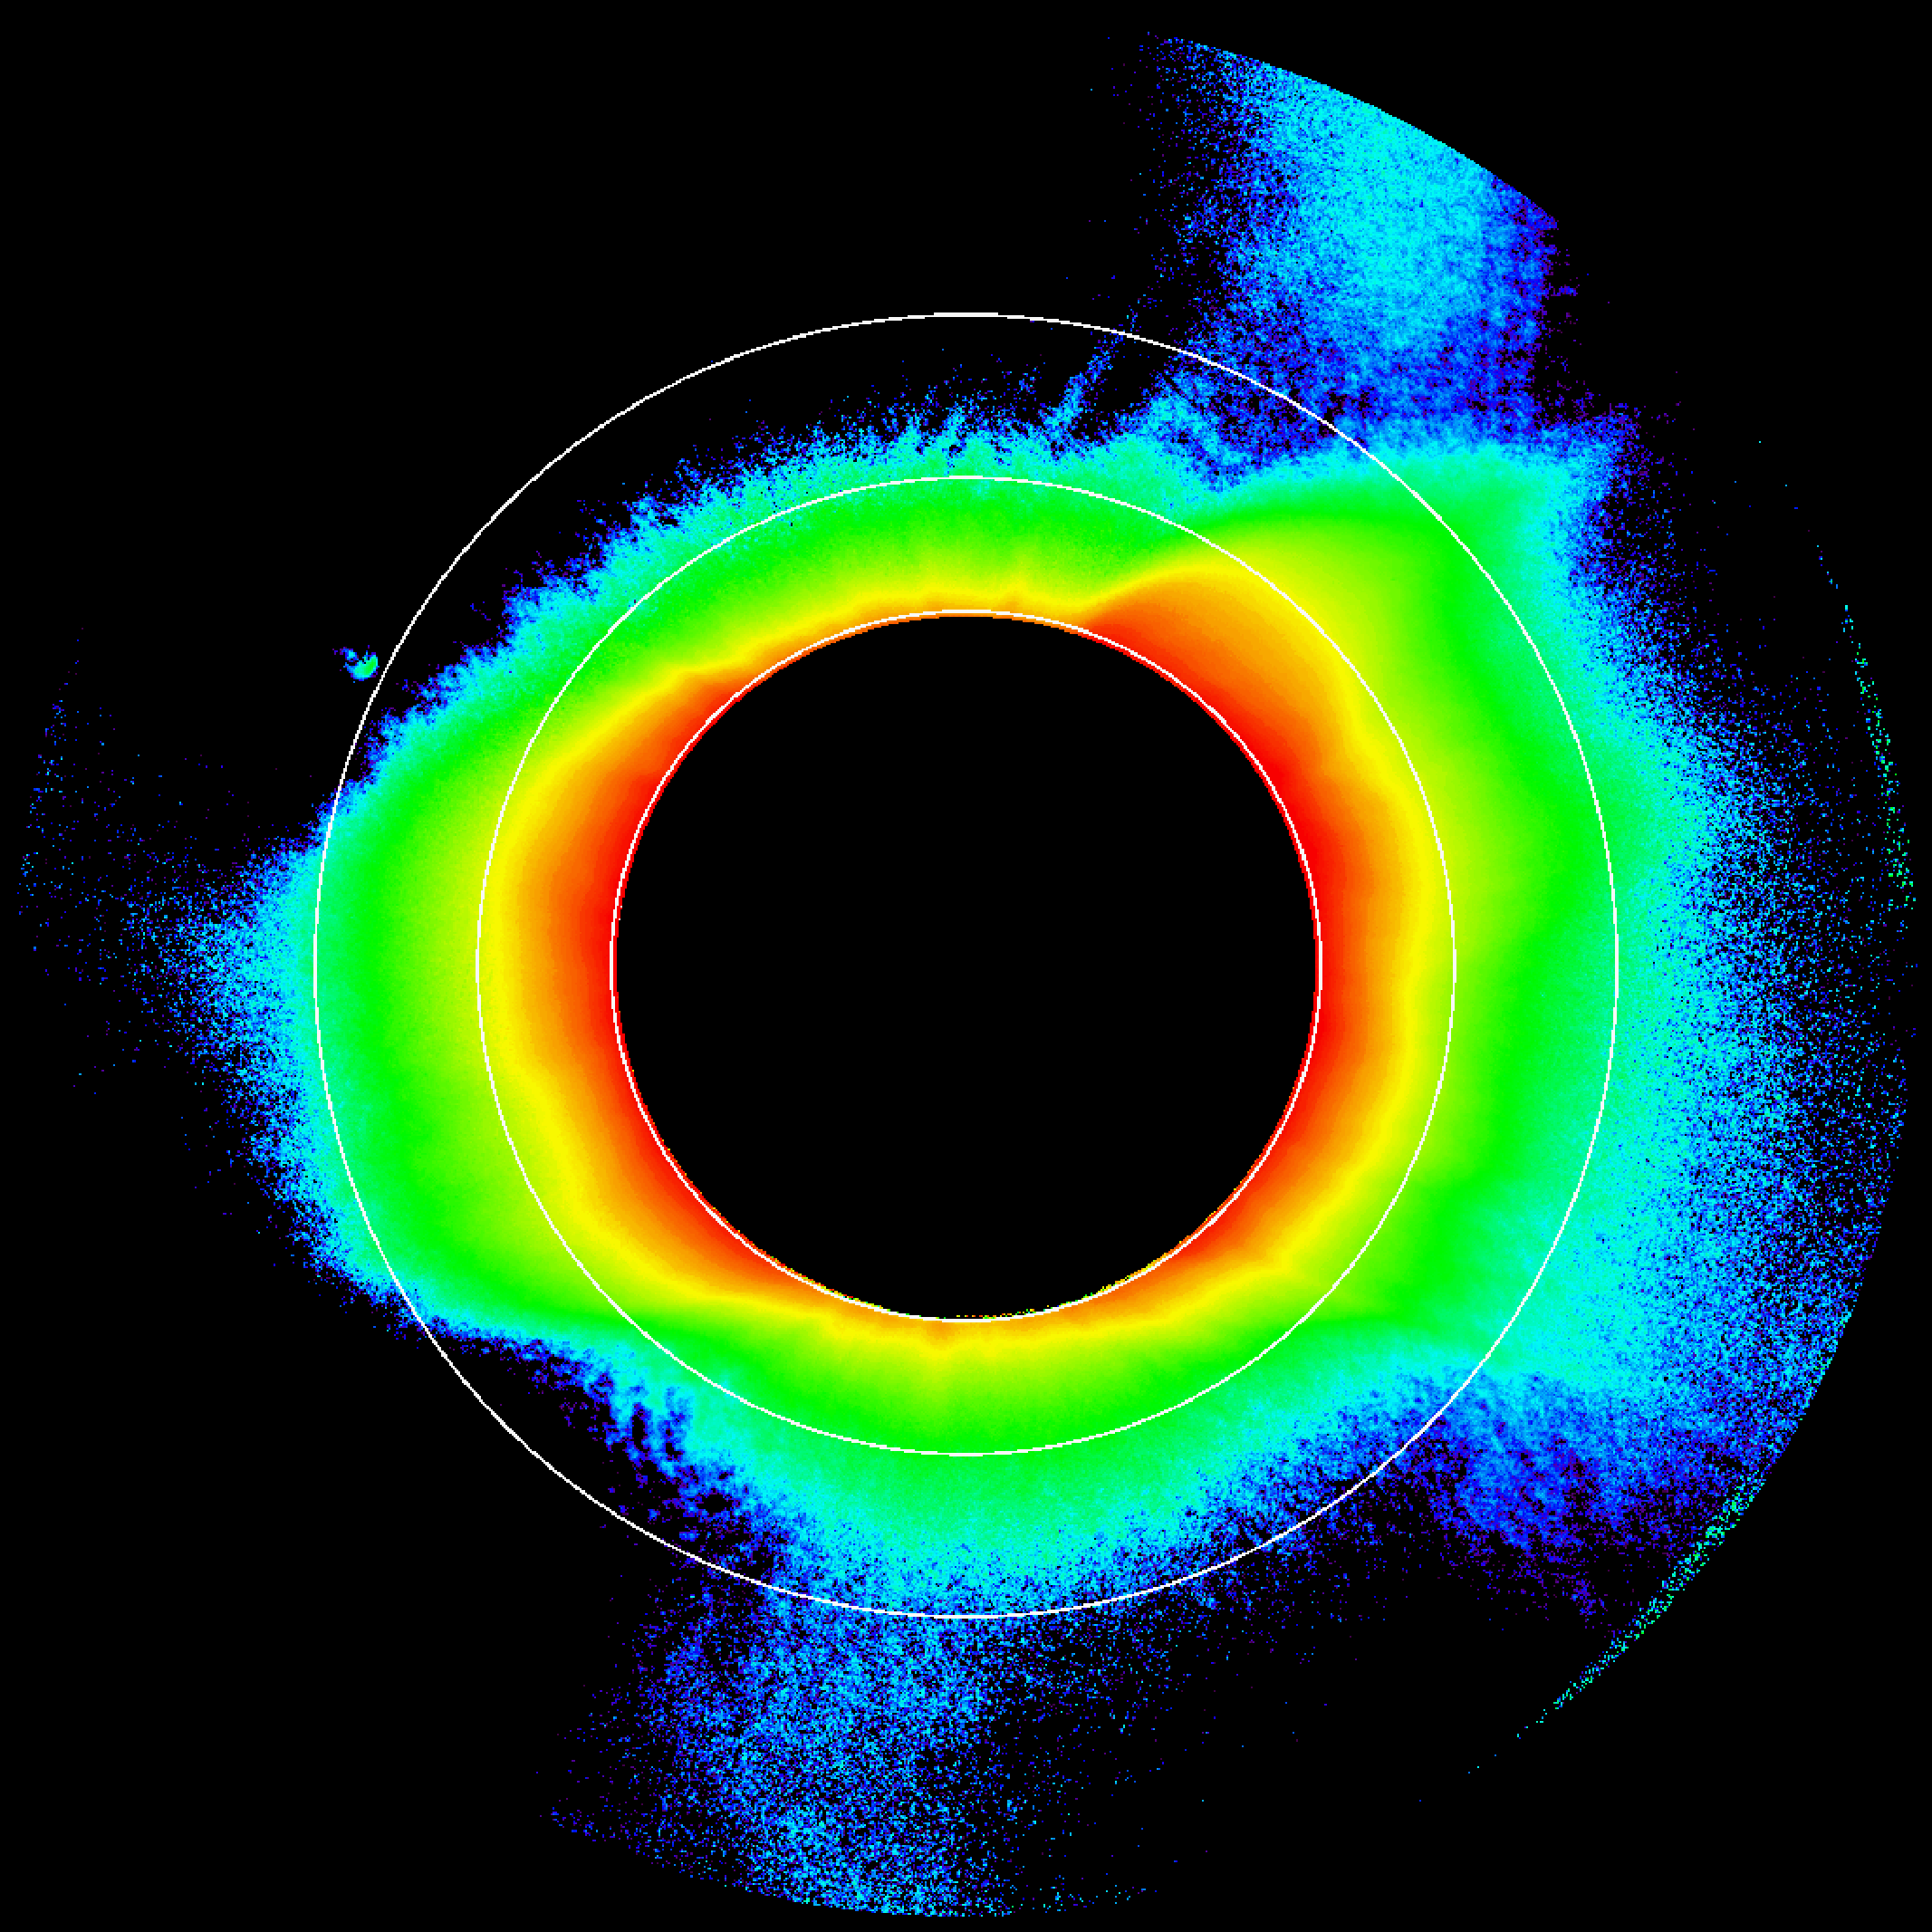
\includegraphics[width=0.68\columnwidth]{20171203_180316_kcor_l1_10min_avg_image.pdf}
  \caption{Example of images used for tomographic reconstruction of the coronal electron density of CR-2198 (see text), both corresponding to 2017 December 03 UT 18:00-19:00. Left panel: SDO/AIA coronal EUV image in the $211~\rm{\AA}$ band. Right panel: HAO/KCOR coronal pB image, with white rings indicating heliocentric heights $1.09, 1.50, \rm{and}\, 2.0~\rm{R}_\odot$.}
  \label{fig_images}
\end{figure*}

While the electron density determined by WL tomography is of an absolute nature \citep{frazin_2010}, that obtained from EUV tomography is dependent on the assumed iron coronal abundance, as well as affected by the so-called coronal filling factor \citep{frazin_2009}. So far, no comparison had been carried out between results obtained with both techniques. Here, the tomographic reconstruction of the coronal electron density for a given period is carried out using both methods and their results are compared for the first time.

\section{Data and Methodology}\label{method}

Carrington rotation (CR-)2198 (2017, December 03 UT 14:37 - December 30	UT 22:25) was selected as target for analysis, a relatively quiet rotation in the declining activity phase of SC-24. Low latitudes were dominated by the equatorial streamer belt, with a complex of active regions (ARs) located in the longitude range $\approx 80^\circ-200^\circ$, and high latitudes were dominated by polar coronal holes (CHs),  

The KCOR and AIA images were obtained for the period 2017, December 03 through December 17, allowing to observe the off-limb corona at all Carrington longitudes. In the case of AIA, images for all the coronal bands $171, 193, \rm{and}\, 211~\AA$ are obtained every 1 hr, and processed with our own tomography data pre-processing tools, which make use of the SolarSoft AIA software in its latest version. In particular, images are averaged over 6 hr long bins, so that a total of about 55 images are used in the end. In the case of KCOR we requested to the HAO team one 10-minute average coronal polarized brightness (pB) image for each day, obtained using its best observational window. 

Figure \ref{fig_images} shows examples of the coronal images used for this work. The left panel shows an AIA coronal EUV image taken in its $211~\rm{\AA}$ band. The right panel shows a KCOR coronal pB WL image. Both images were taken nearly-simultaneously on 2017 December 03 UT 18:00-19:00. This is roughly the beginning of CR-2198, so the longitude of the disk center in these images is $\approx 0^\circ$, so the ARs are not seen and the images are dominated by the quiet sun streamer belt and the CHs.

Both the WL and EUV tomographic reconstructions were performed on the same resolution, with computational voxels having uniform radial size of $0.01~\rm{R}_\odot$ and angular size of $2^\circ$ in both latitude and longitude. Solutions were computed with a 3D regularization scheme.

\section{Results}

For the specific data sets of this rotation, the coronal electron density structure was reconstructed in the height range $1.02-1.20~\rm{R}_\odot$ from EUV tomography, and $1.09-1.80~\rm{R}_\odot$ from WL tomography. Figure \ref{fig_maps} shows Carrington maps of both reconstructions at heliocentric height $r=1.105~\rm{R}_\odot$. 

The white boxes in the maps indicate two regions selected for quantitative comparison. The region in the Southern hemisphere is a high-density quiet Sun region within the equatorial streamer belt. The region in the Northern hemisphere is a lower density region at subpolar latitudes in the northern CH.

The quantitative comparison of the electron density determined from both tomographic analysis at each computational voxel of the two selected regions is shown in Figure \ref{fig_analysis}. For each region, the top panel shows the histogram of the ratio of electron density as determined from both tomographic analysis for all voxels within the common reconstructed coronal volume, i.e. in the range of heights $1.09-1.20~\rm{R}_\odot$.
For each region, the bottom panel shows the average radial dependence of the electron density determined from both analysis.

\begin{figure*}[t]
  \centering
  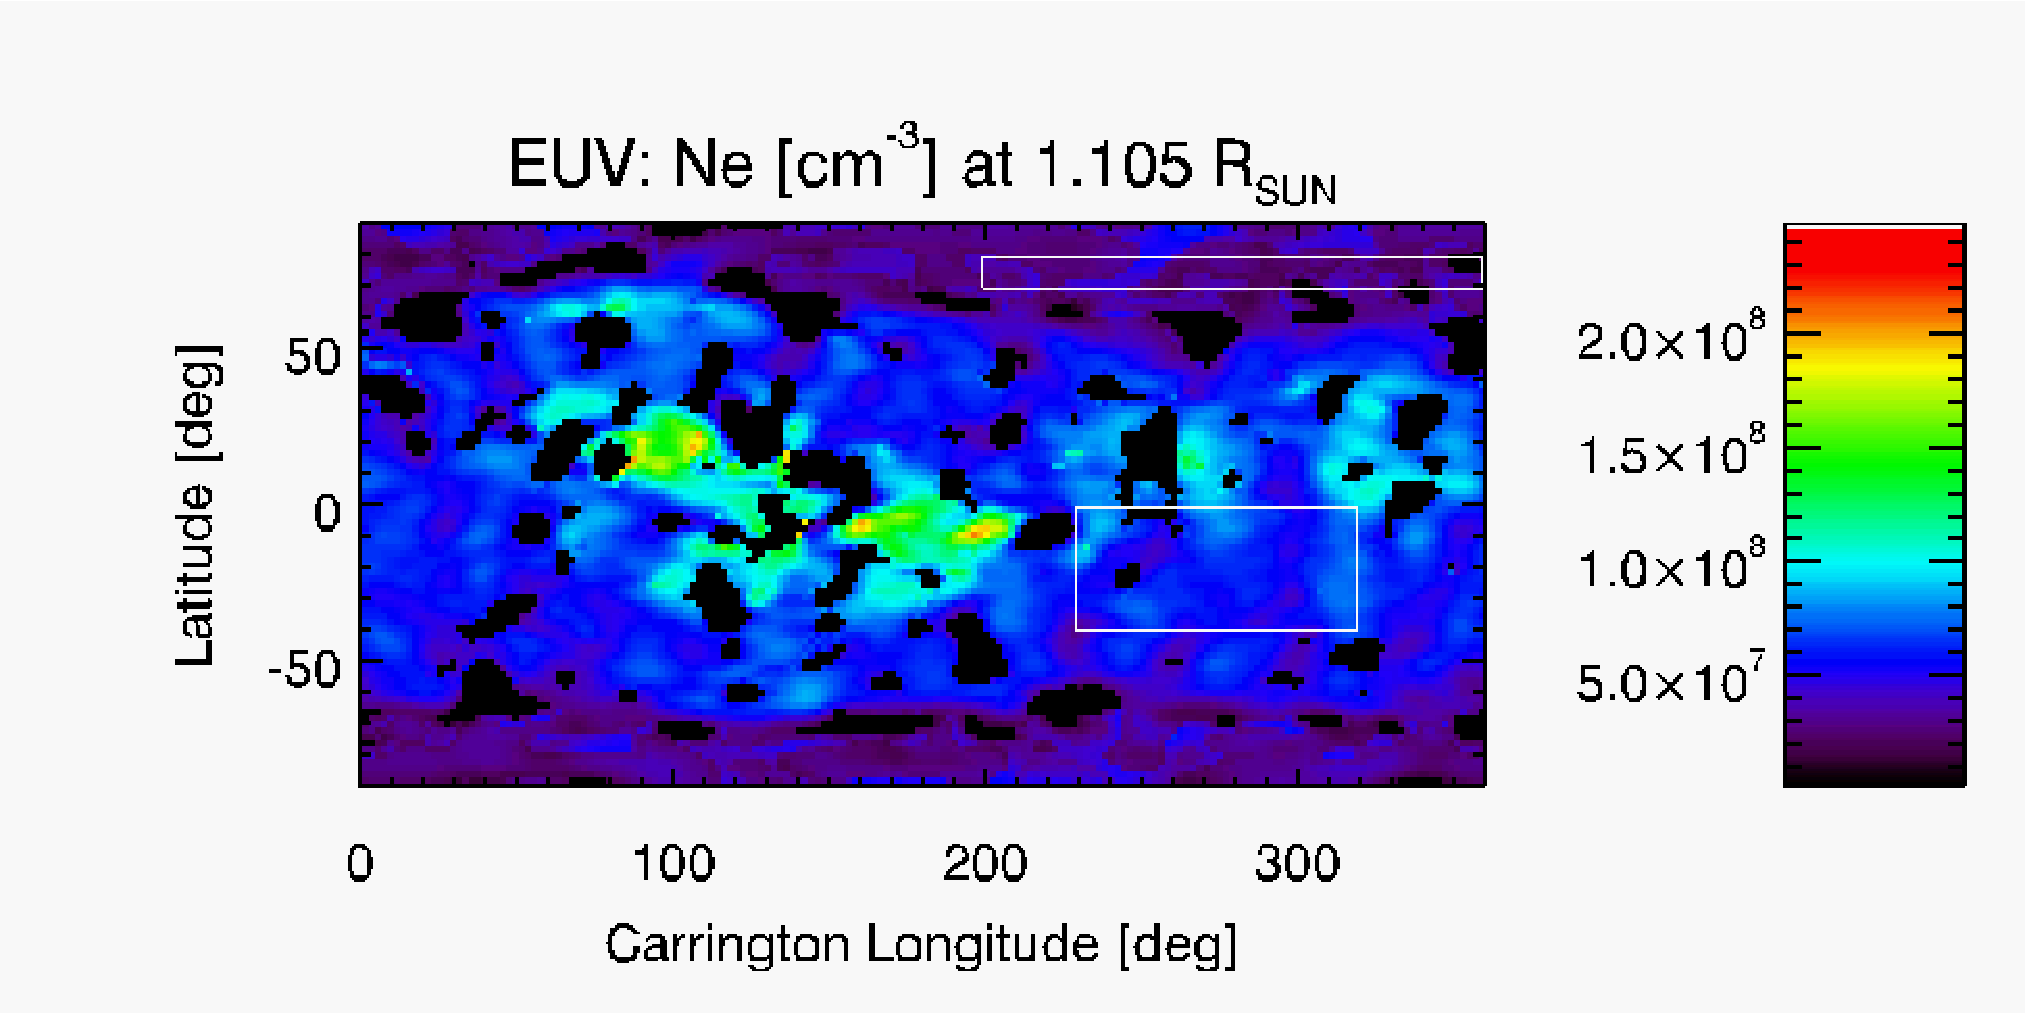
\includegraphics[width=\columnwidth]{map_ne_aia.pdf}
  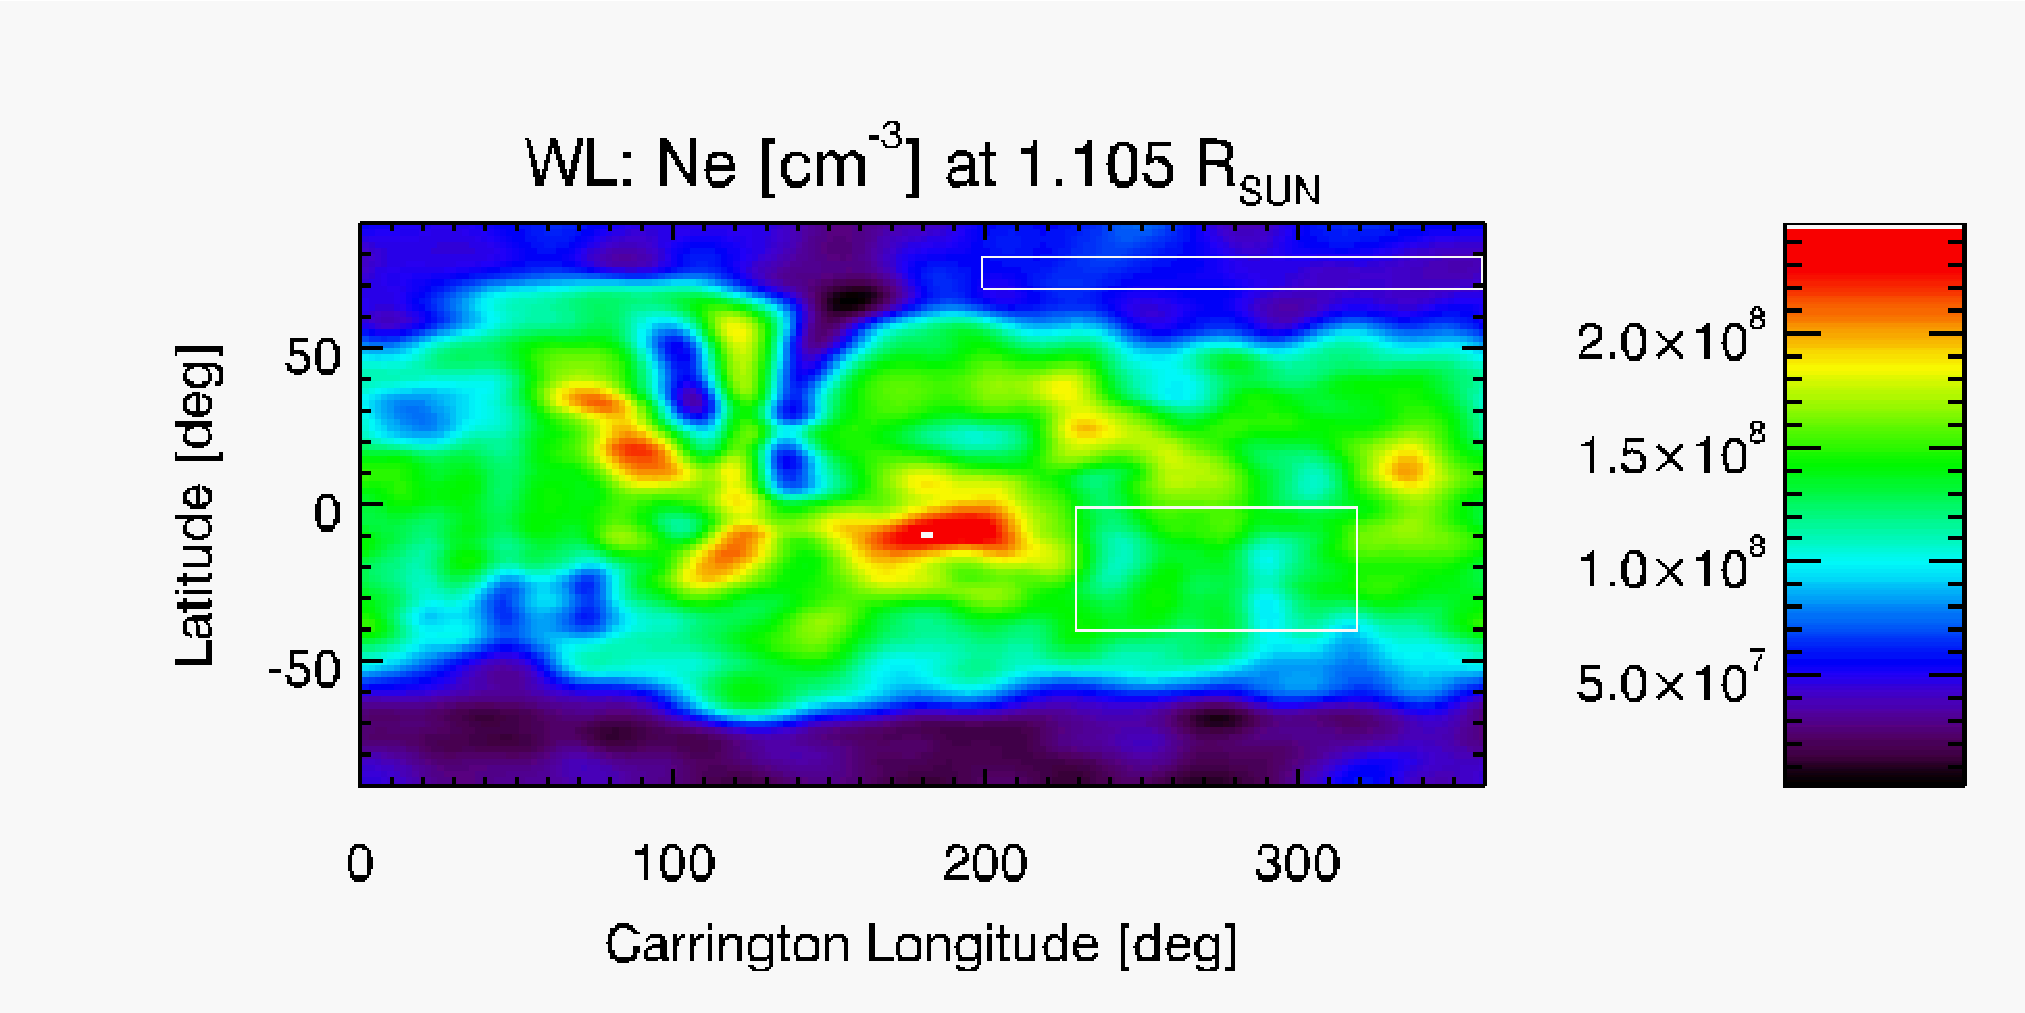
\includegraphics[width=\columnwidth]{map_ne_kcor.pdf}
  \caption{Example of results of the tomographic reconstruction of the electron density of the solar corona for CR-2198. Carrington maps of the reconstructed electron density are shown at heliocentric height $r=1.105~\rm{R}_\odot$. Left panel: reconstruction based on EUV data. Right panel: reconstruction based on WL data. The white boxes indicate two ranges of longitudes and latitudes selected for quantitative comparison (see text).}
  \label{fig_maps}
\end{figure*}

\begin{figure*}[h!]
  \centering
  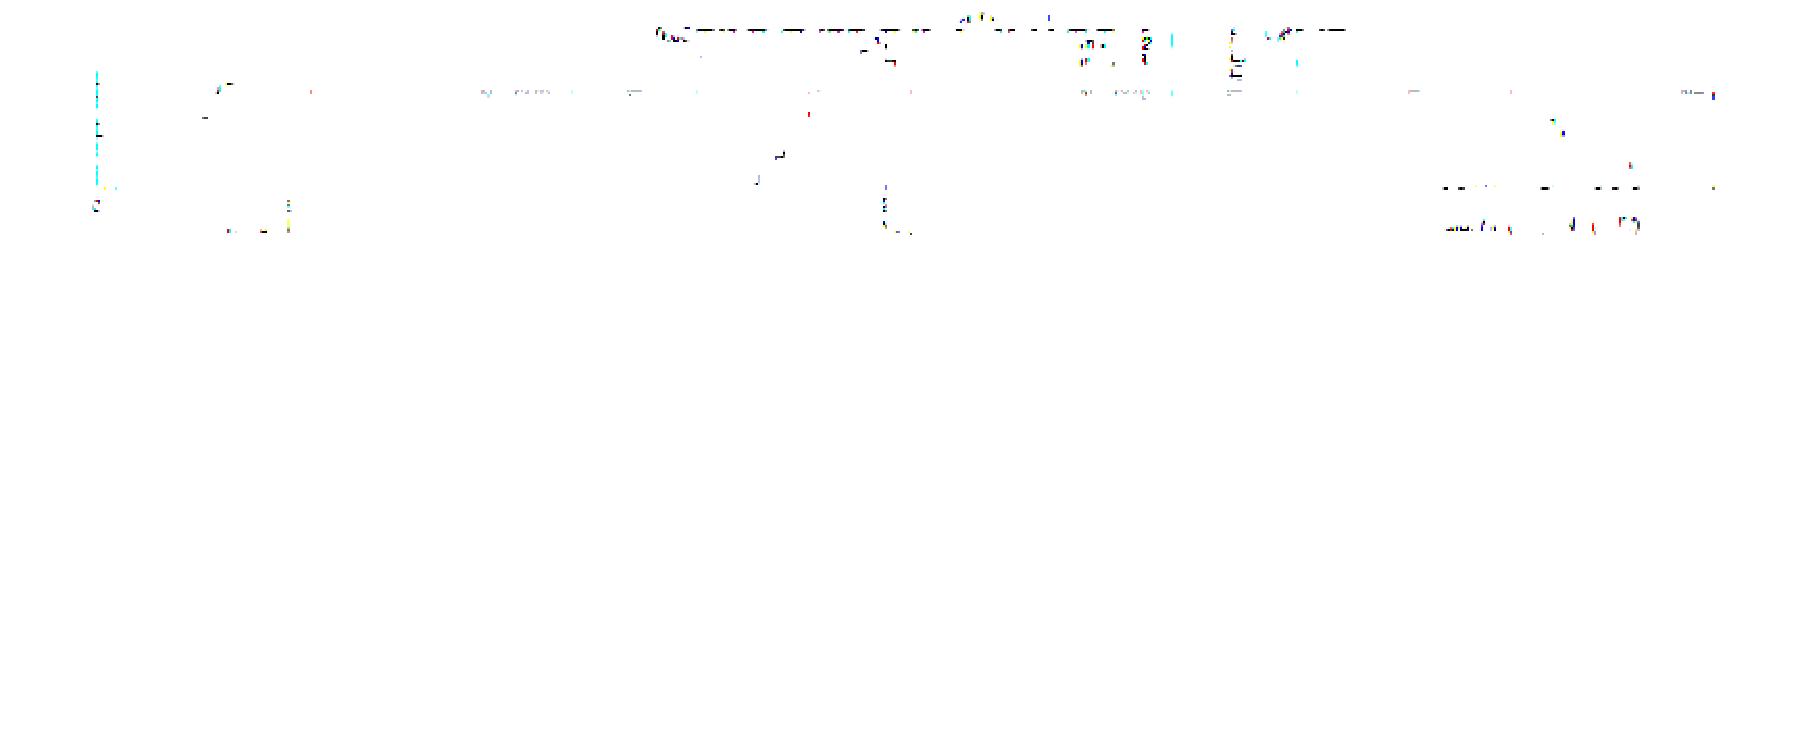
\includegraphics[width=\columnwidth]{comparison_quiet_region.pdf}
  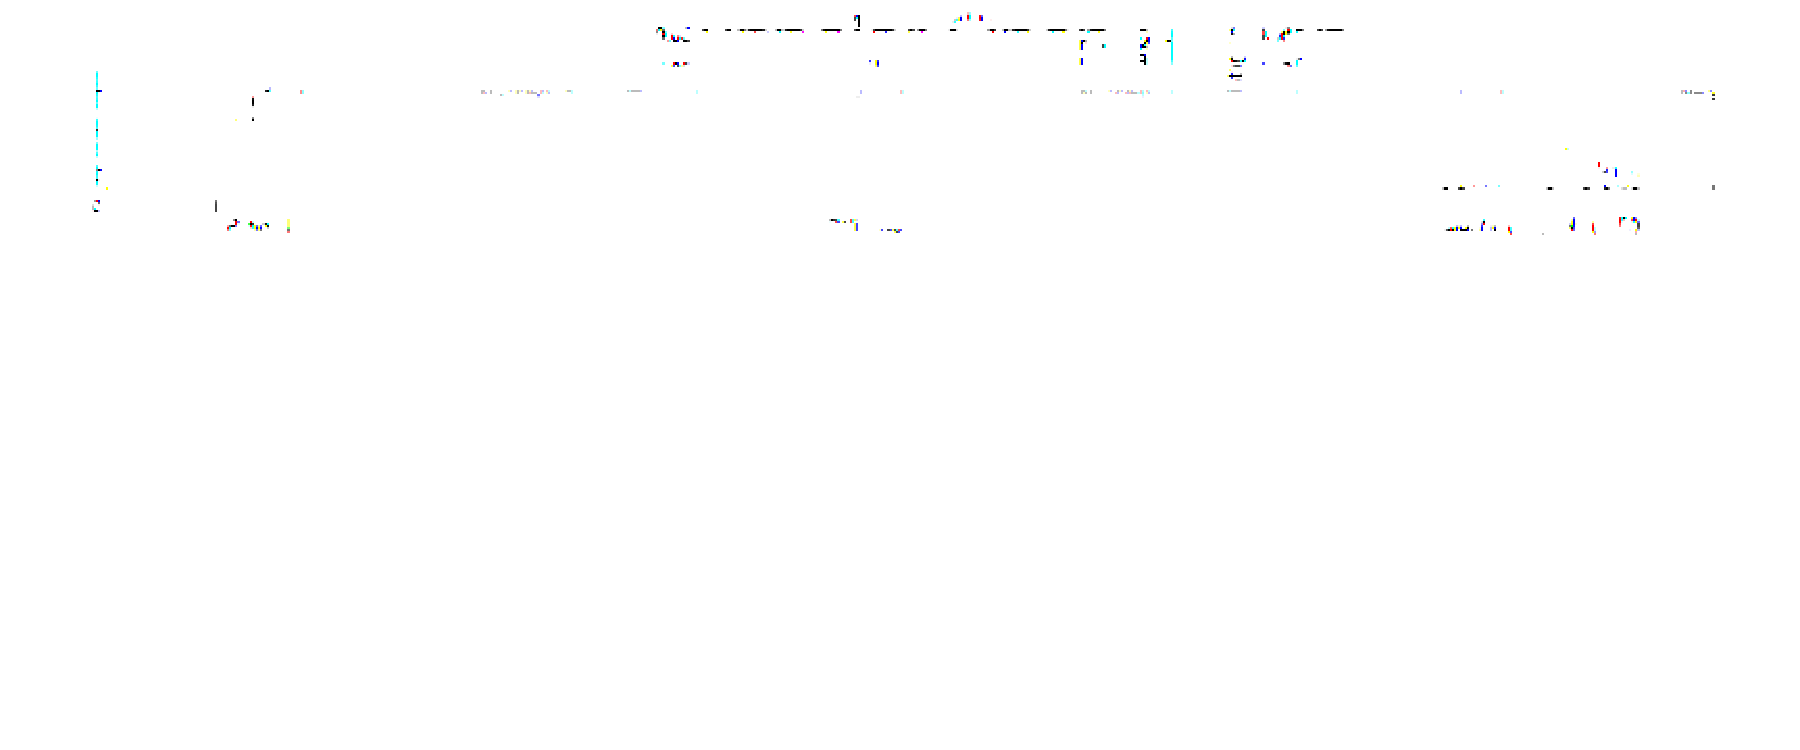
\includegraphics[width=\columnwidth]{comparison_open.pdf}\\
  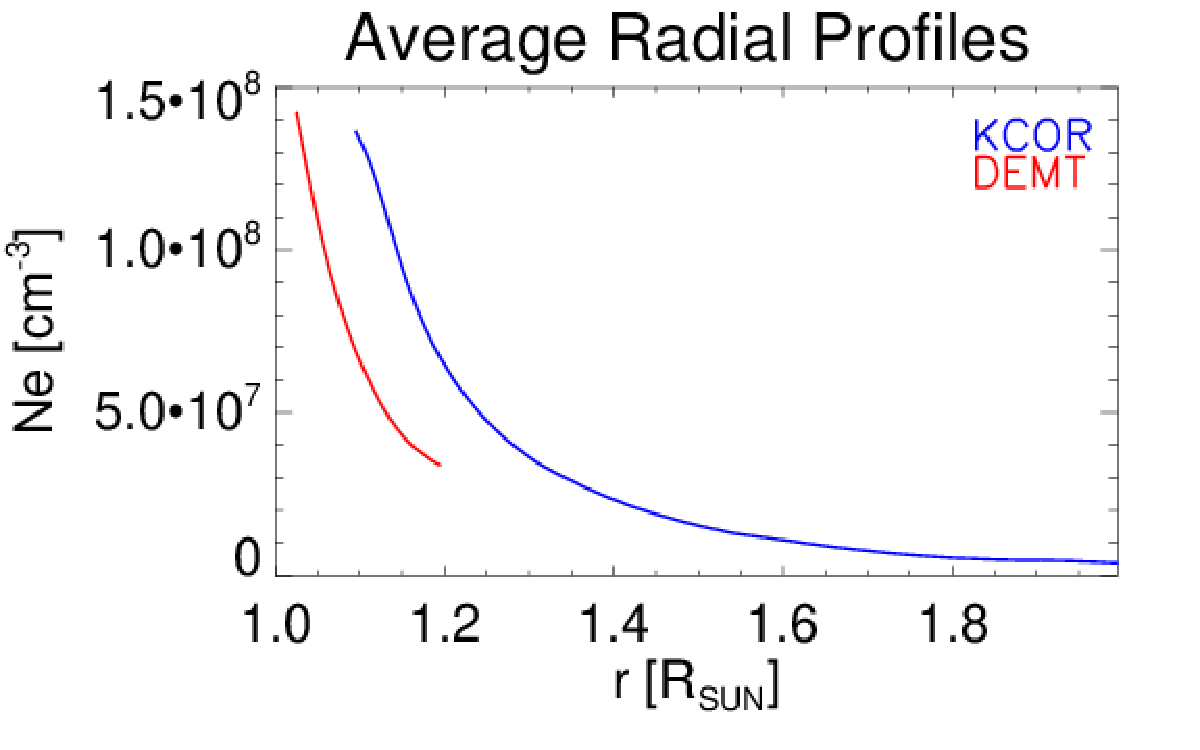
\includegraphics[width=0.75\columnwidth]{Average_Radial_Profiles_KCOR-Tom_vs_DEMT_CR2198_Hh_l45_kcor_subreg-Quiet-region1.pdf}
  \hskip 2cm
  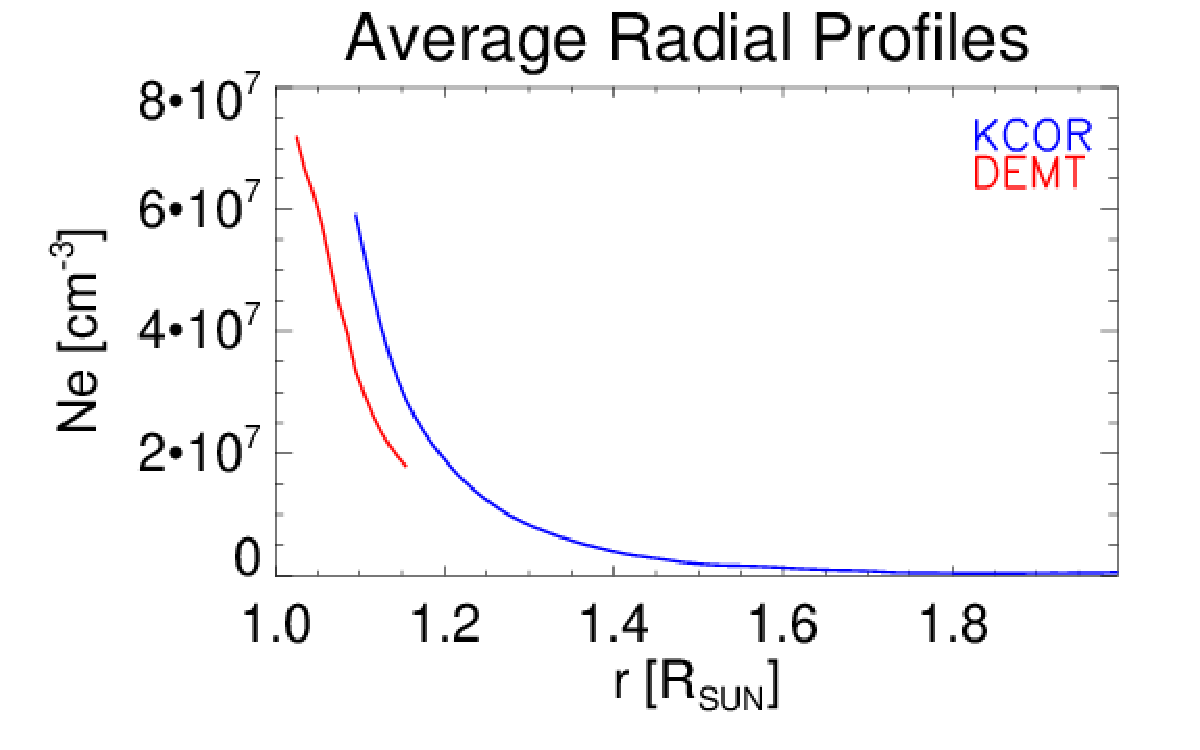
\includegraphics[width=0.75\columnwidth]{Average_Radial_Profiles_KCOR-Tom_vs_DEMT_CR2198_Hh_l45_kcor_subreg-Open-region_N.pdf}
  \caption{Quantitative comparison between the results of the two tomographic reconstructions of the coronal electron density of CR-2198 in the two selected regions indicated in Figure \ref{fig_maps}. Left panels show the results in the quiet sun region of the southern hemisphere within the streamer belt, and right panels show the results in the subpolar open region within the northern CH. For each region, the top panel shows the histogram of the ratio of the electron density value obtained in each computational voxel from the WL and EUV tomographic analysis. For each region, the bottom panel shows the average radial profile of the electron density based on the EUV (red) and WL (blue) tomographic reconstructions.}
  \label{fig_analysis}
\end{figure*}

\section{Discussion and Future Work}

The coronal electron density determined from WL tomography is systematically larger than that determined from EUV tomography. The characteristic (median) WL-to-EUV electron density ratio is $\sim 2.0$ in the quiet sun streamer belt region and $\sim 1.6$ in the subpolar region within the CH.

This difference may be partly explained by the fact that the KCOR data is affected by the sky brightness which was not subtracted in the specific data set used for this first work, as the required procedures were being revised by the HAO team at the moment of this analysis. Once applied a sky subtraction, the electron density as determined from WL tomography will systematically decrease. However, once corrected a difference is still expected to remain in the electron density as determined from the two analyses. In that case, systematic differences can be attributable to physical factors. 

Firstly, the EUV emissivity determined at each voxel from tomographic analysis is proportional to the local mean squared electron density, i.e. $\Eeuv \propto \AvgNE2 = f\,\AvgNe^2$, where the \emph{filling factor} is here defined as $f\equiv\AvgNE2 / \AvgNe^2 > 1$. As the WL emission is due to Thompson scattering, its voxel emissivity is proportional to the local average electron density, i.e. $\Ewl \propto \AvgNe$. Then: $\AvgNe_{\rm{WL}} / \AvgNe_{\rm{EUV}} \propto \sqrt{f}$. 

If differences in the results are solely attributed to the filling factor $f$, then $f\sim 4.0$ the quiet sun region of the streamer belt, and $f\sim 2.5$ in the subpolar region of the CH. As for any probability distribution, $\SigmaNe^2 \equiv \rm{Var}(N_e) = \AvgNE2 - \AvgNe^2 = \AvgNe^2 \, (f-1)$, then $\SigmaNe / \AvgNe = \sqrt{f-1}$. With this interpretation, where $f$ is larger (quiet sun region) the electron density probability distribution has a larger variance.

Secondly, the EUV emmisivity determined from tomography is proportional to the assumed iron coronal abundance $[\rm{Fe}]$. As a result, the EUV tomography estimate of the average squared electron density scales as $\AvgNE2 \propto 1/[\rm{Fe}]$ \citep{frazin_2009}.

The work here summarized is a first step towards development of a new methodology capable of jointly determining the coronal 3D distribution of the electron density and temperature, as well as the filling factor and iron abundance. The technique, dubbed multi-instrument tomography (MIT) and currently under development, will involve joint analysis of tomographic products based on data provided by multiple instruments. These include white-light coronagraphs, EUV telescopes, and visible emission line coronagraphs. In particular, MIT will attempt to combine KCOR and AIA data, with that to be provided by the (soon to be operative) Upgraded Coronal Multichannel Polarimeter (UCoMP) instrument \citep{landi_2016}.

\bibliographystyle{baaa}
\small
\bibliography{baaa61a_dglloveras}
 
\end{document}
